\section{APPENIX STUFF}\label{appendix_basic_hop}
Hi I'm your Appendix

%%%%%
\section{Instructions on Use of Interface}
[NOTE: from https://www.metaculus.com/help/faq/#howscore ]
Here are the instructions provided to participants regarding how to enter a prediction.

"How do predictions and points work for numerical questions?
Binary questions resolve to either 'yes' or 'no', but numerical questions resolve to a number. Therefore, when you make a prediction on a numerical question, you need to specify a probability for each possible outcome (that is, assign a probability density function). There are an infinite number of such functions, but to make life a little bit easier we restrict predictions to a mixture of up to 5 logistic distributions. You can adjust the center, width and weight of each component of the mixture using the sliders on the question pages.
Here are the key things you need to know, with more details below.
	1.	You should put the center of your distribution at what you think is the most likely value, then adjust the width of the distribution so that you attribute better than even odds to the true number falling into your range.
	2.	Making your distribution wider or narrower reflects your confidence in the central value you've specified, and decides the stakes: a narrower distribution gives more points if your central value is right, but makes you lose more if it's wrong.
	3.	As for binary questions, points are awarded both for being right and for being more right than the community. The points "on the line" will change over time, and the score you are awarded is time averaged over the time during which the question is open.
	4.	Some numerical questions restrict the possible resolutions to lie within a certain range. If the resolution falls outside of that range, then the question resolves ambiguously and no one receives any points. Other questions allow open-ended ranges, and you can assign probability to an out-of-bounds resolution by moving your distribution to the edge of the range."









%%%%
%%SCRAP BELOW HERE
%%%%

%Figure \ref{fig:TheoryPosteriorDists} 

%\begin{figure}
%    \centering
%    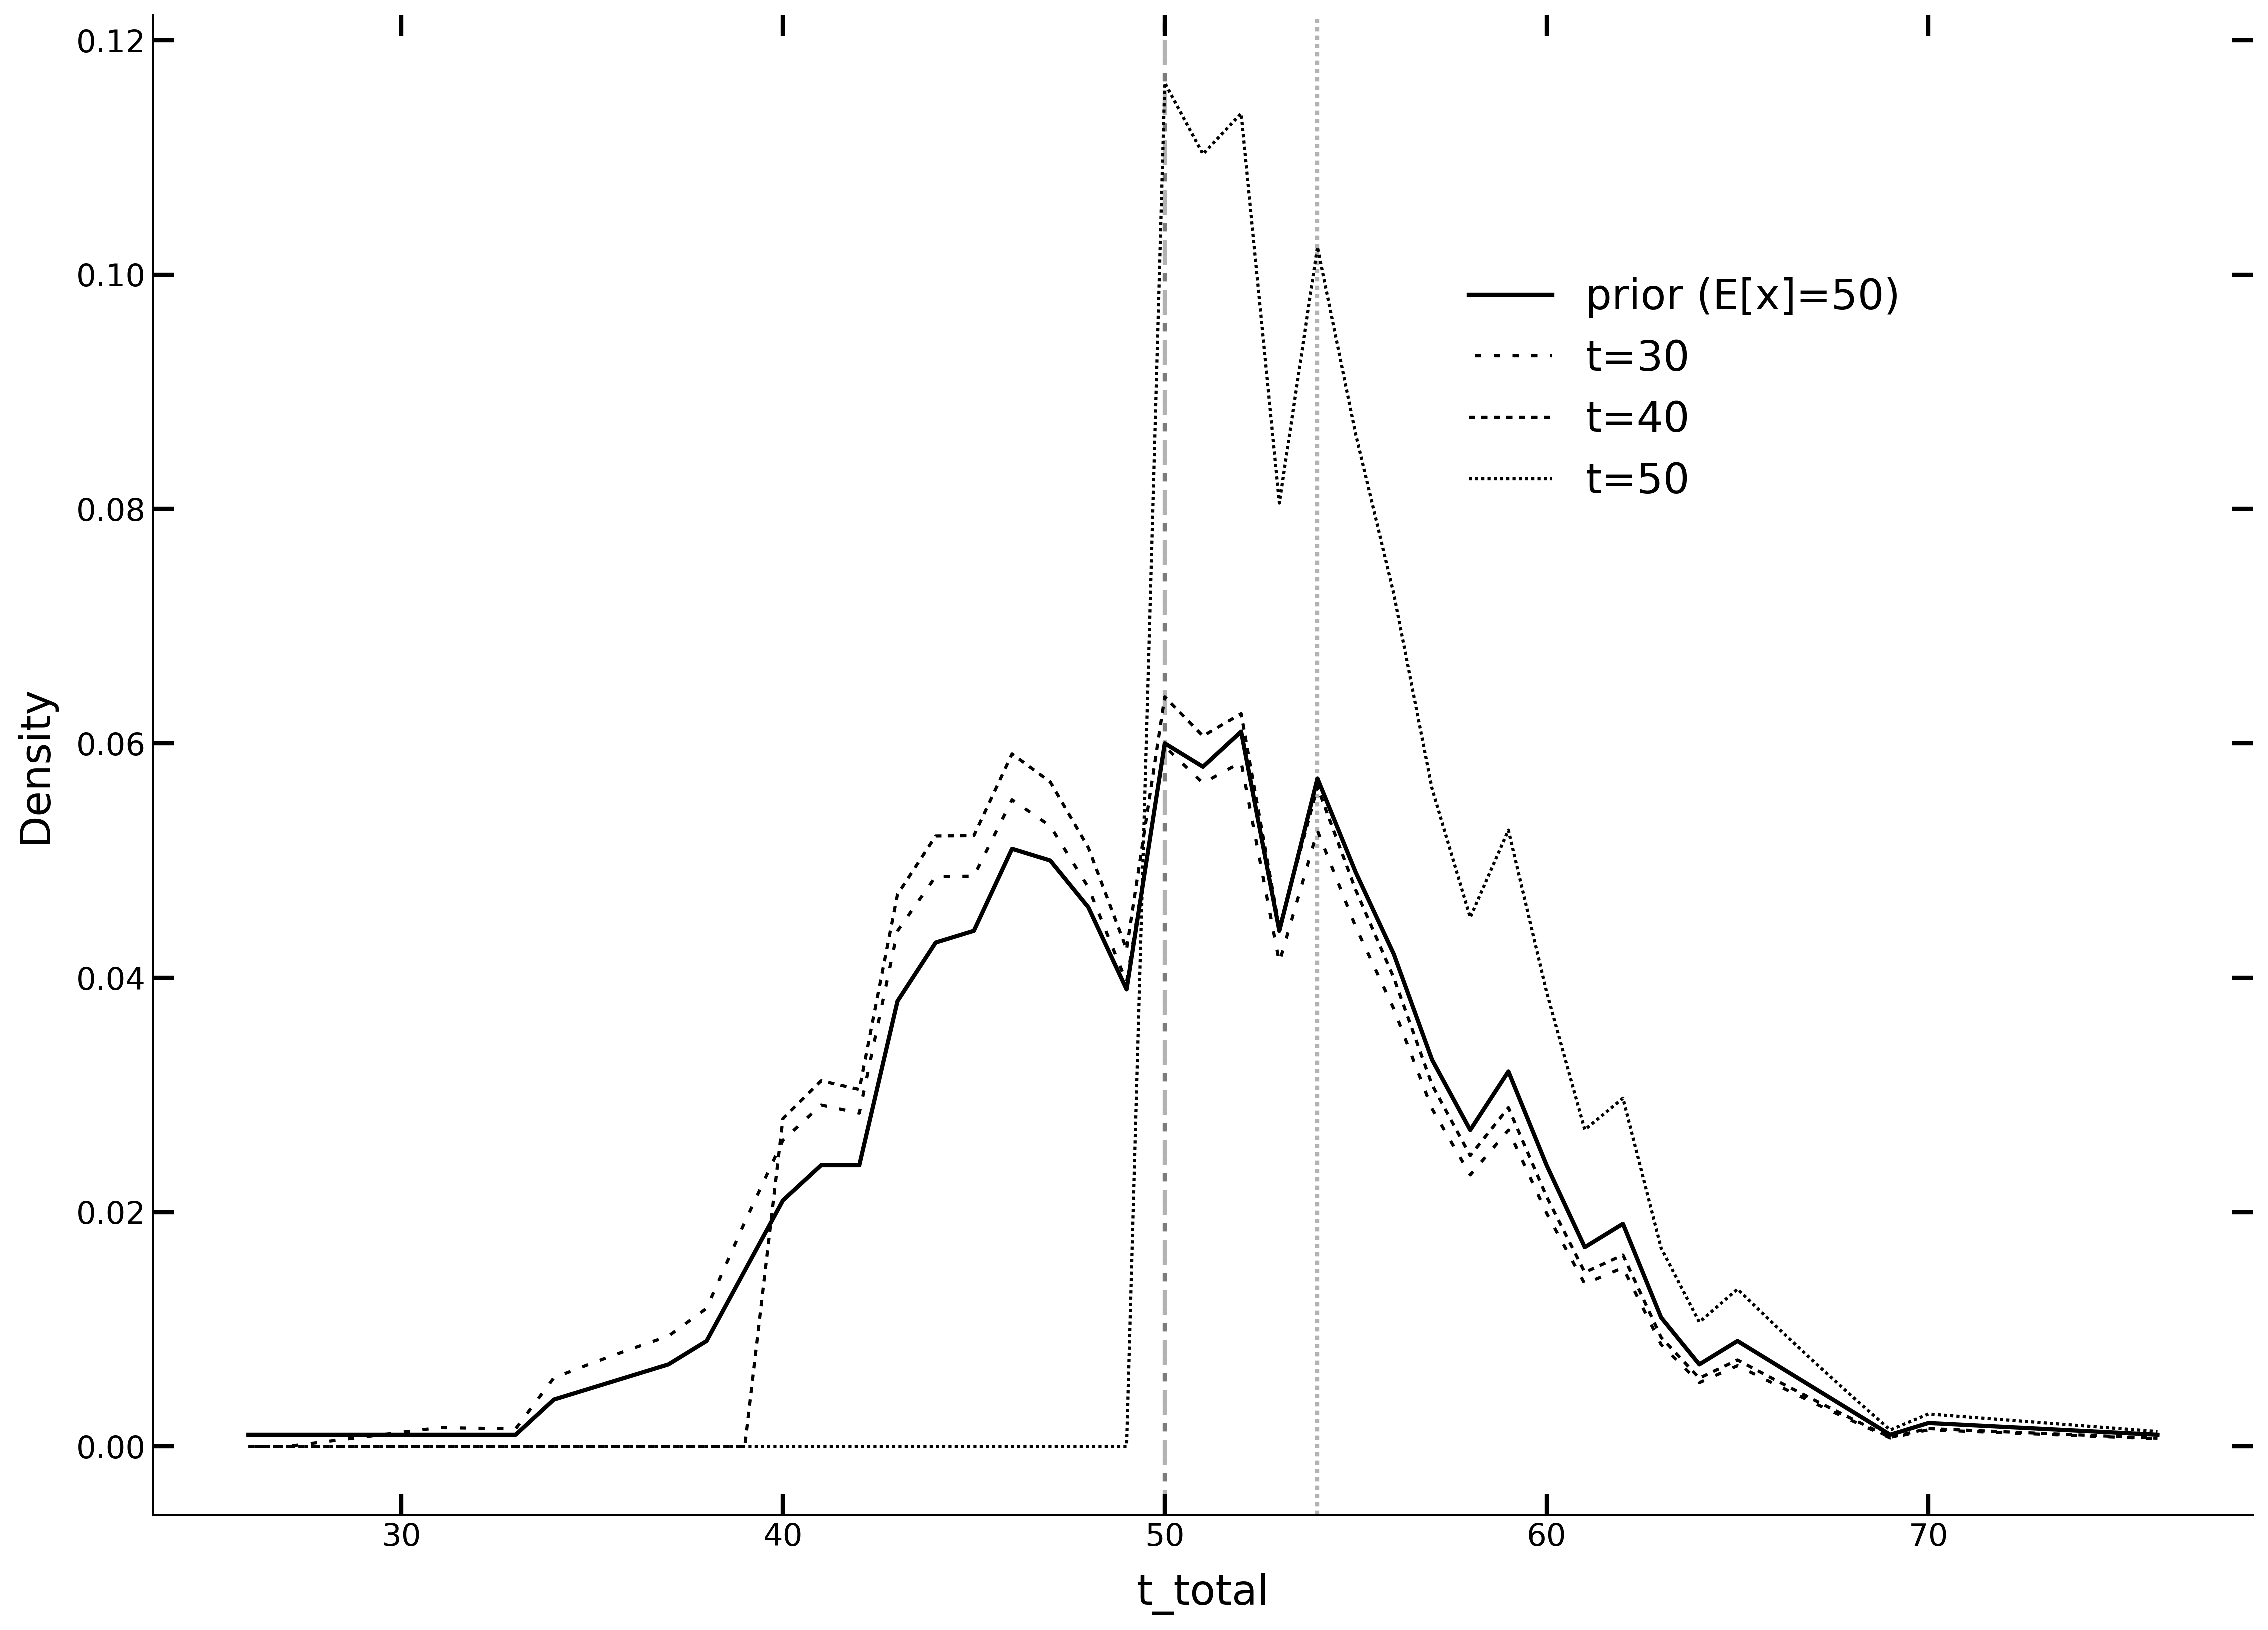
\includegraphics[width=\linewidth]{Figures/TheoryPosteriorDists_1.png}
%    \caption{
%    This figure depicts stuff
%    }
%    \label{fig:TheoryPosteriorDists}
%\end{figure}



%Figure \ref{fig:PriorShift2} visualizes the prediction of the theory as $t_i$ approaches the median of a prior.  
%\begin{figure}
%    \centering
%    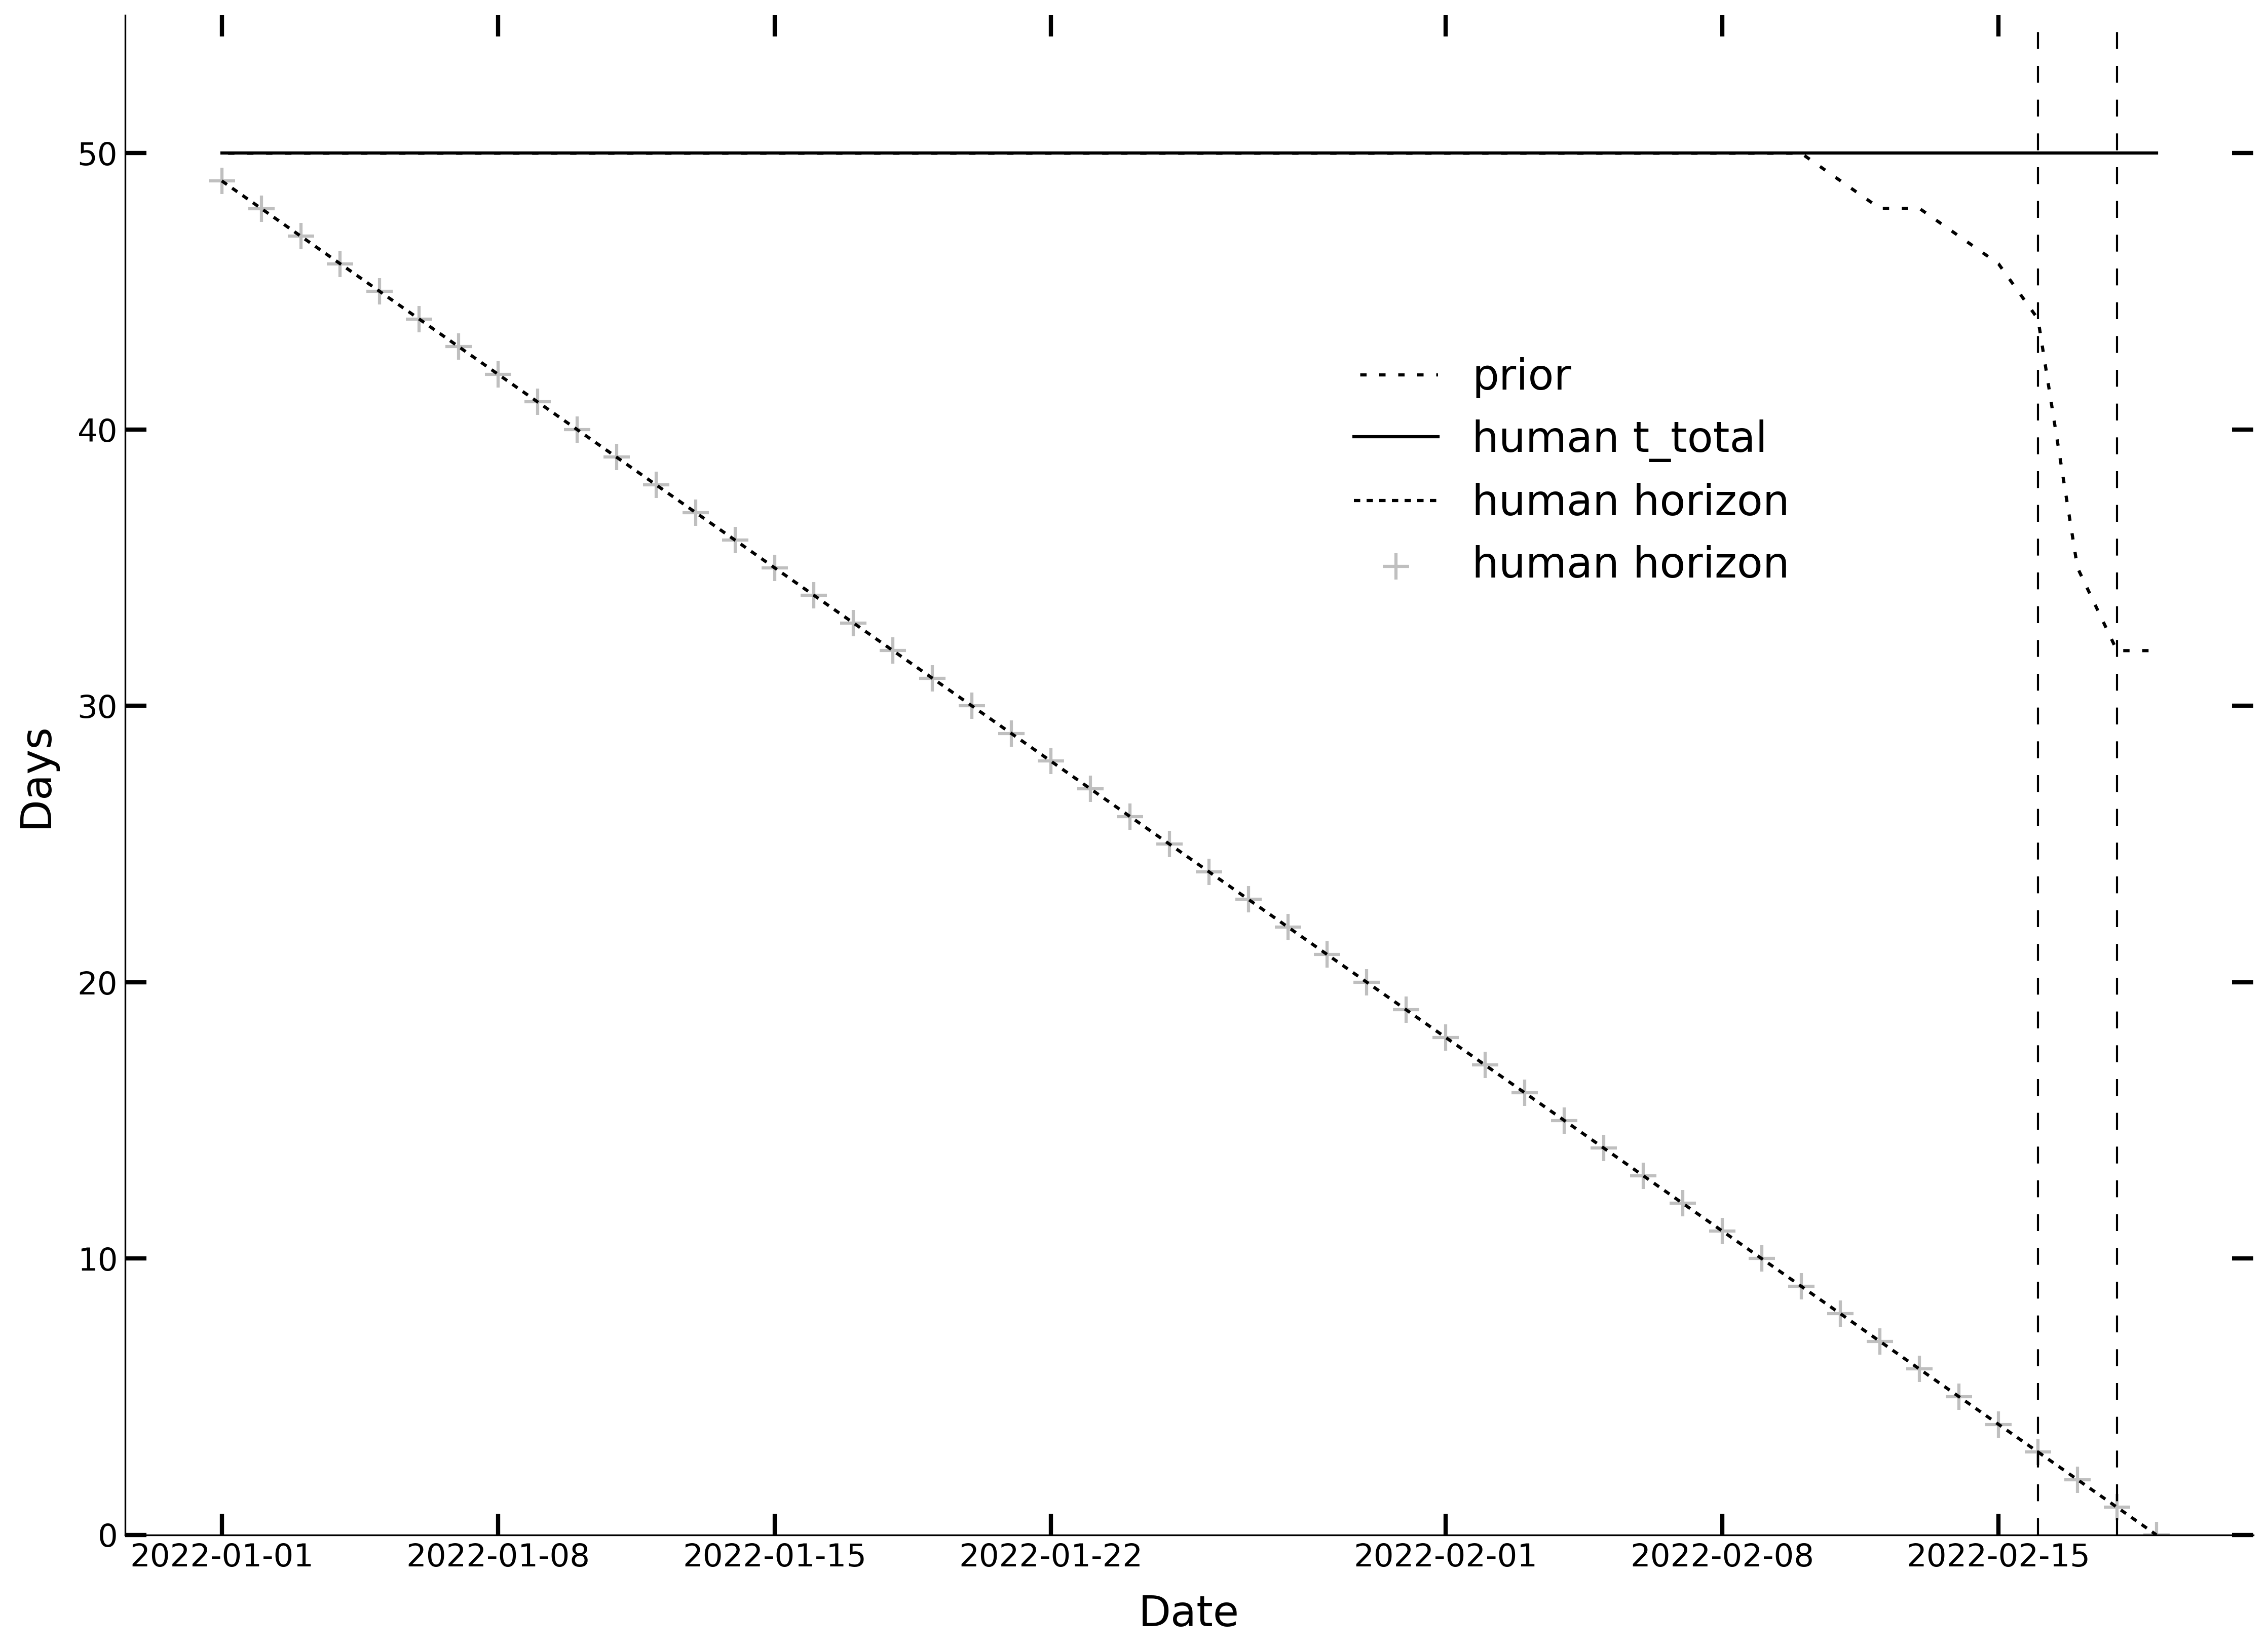
\includegraphics[width=\linewidth]{Figures/Theory_PriorShift_2.png}
%    \caption{hi
%    }
%    \label{fig:PriorShift2}
%\end{figure}

%Figure \ref{fig:PriorShift1} visualizes the prediction of the theory as $t_i$ approaches the median of a prior.  
%\begin{figure}
%    \centering
%    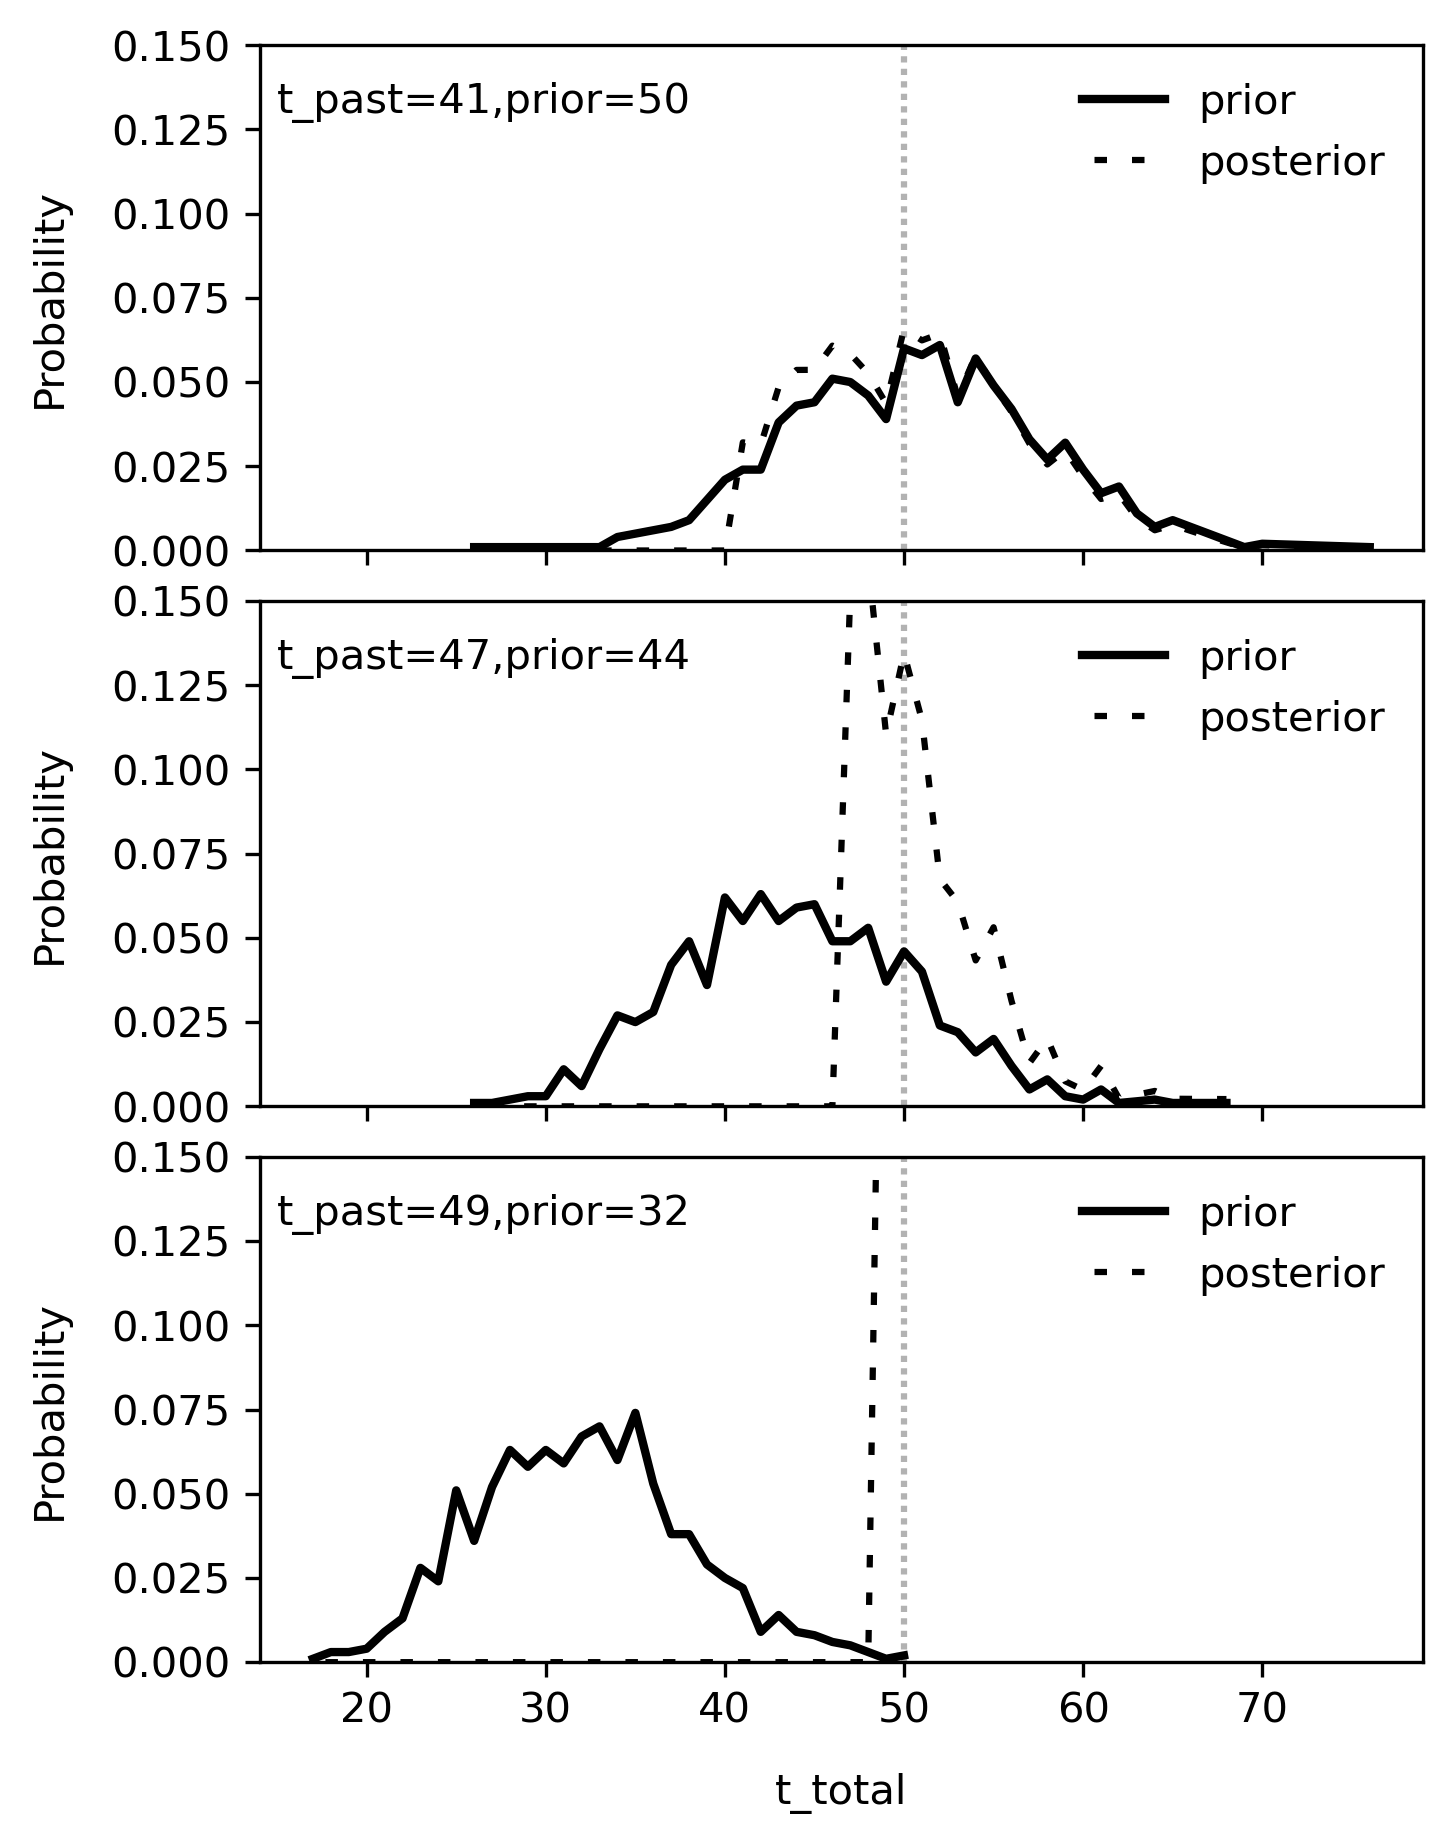
\includegraphics[width=\linewidth]{Figures/Theory_PriorShift_1.png}
%    \caption{hi
%    }
%    \label{fig:PriorShift1}
%\end{figure}

%\begin{equation}\label{posteriordist}
%    \sum_{i=1}^{max} P(t_{total_{i}} \vert t)
%\end{equation}